\documentclass[tikz]{standalone}

\begin{document}

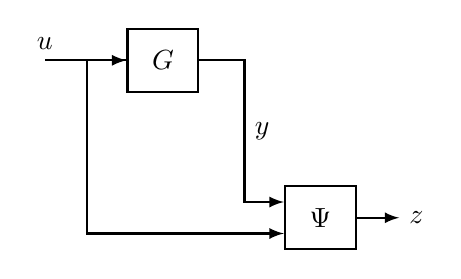
\begin{tikzpicture}[thick,>=latex,auto]
  \tikzstyle{block}=[draw,rectangle,inner sep=2mm,minimum width=0.9cm,minimum height=0.8cm]
  \def\dx{1.2}	% width of u,y loops
  \def\dy{1.3}	% v-dist of G and phi blocks
  \def\dk{0.9}	% separation of Psi attachments
  \def\dz{0.7}	% v-dist of Psi block
  \node[block] (G) at (0,0) {$G$};
  \path (G) + (-\dk,0) coordinate (uu);
  \node[block] (psi) at (2,-\dy-\dz) {$\Psi$};
%   \draw[<-] (psi.west) + (0,.2) -| (yy);
%   \draw[<-] (psi.west) + (0,-.2) -| (uu);

  \draw[<-] (G) -- +(-1.5,0) node[anchor=south] {$u$};
  \draw[<-] (psi.west) + (0,.2) -- +(-0.5, 0.2) |- node[swap, pos=.25]{$y$} (G.east);
  \draw[<-] (psi.west) + (0,-.2) -- +(-2.5, -0.2) |- (G.west);
  \draw[->] (psi) -- +(1,0) node[anchor=west] {$z$};
\end{tikzpicture}

\end{document}
